\section{Généralité}

Dans un premier temps, l’équipe va travailler comme un seul et même groupe. Puis, dans le but de mener au mieux ce projet, chacun aura un rôle spécifique et donc des responsabilités dans un domaine donné afin de paralléliser les tâches.

\section{Rôles}

\subsection{Chef de Projet}

Le chef de projet sera Paul Dautry.
Il assurera que le projet sera mené à bien et que son déroulement sera optimal. Toute l’équpe lui fera confiance afin qu’il identifie et redistribue les différentes tâches en fonction des compétences de chacun. Son rôle sera également de maintenir le tableau de bord à jour et d’établir le planning. En cas de dépassement des délais ou de mauvaise gestion de notre temps, il sera de son devoir de redresser la barre pour que le projet avance de façon rapide et efficace.

\subsection{Responsable Qualité}

Antoine Chabert sera notre responsable qualité : ce rôle non négligeable permettra à tous les documents du projet d’être cohérents, aussi bien du point de vue de la forme qu’au niveau du contenu. Des documents tels que le Plan d’Assurance Qualité répondent exactement à cette demande, permettant à tous nos livrables d’être homogènes.
    Il communiquera en permanence avec tous les membres de l’équipe afin d’assurer la justesse et la cohérence de leurs documents.

\subsection{Experts}

Enfin, plusieurs experts seronts assignés à différentes tâches du projet.

\subsubsection{Responsable modélisation/processus}

Estelle Lepeigneux sera responsable modélisation/processus. Ce responsable effectura de nombreuses démarches de conception, d’urbanisation et d’architecture d’entreprise. Il devra s’assurer que la refonte des processus de Spie est optimale et adaptée aux évolutions des métiers de l’entreprise. Il devra également garantir que les solutions construites répondent aux attentes organisationnelles et informatiques et suivent un modèle adapté et respectant les critères du processus de modélisation.

\subsubsection{Expert ERP}

Hugues Verlin sera expert ERP. Il aura la charge de contrôle la réalisation du modèle cible basé sur les fonctions standard SAP sélectionnées. Ledit modèle sera documenté afin de répondre au mieux aux besoins de Spie. L’expert devra veiller au respect des “bonnes pratiques”.

\subsubsection{Expert Métier}

L’expert métier sera Pierre Jarsaillon. Il fera bénéficier l’équipe de sa compétente fonctionnelle sur les processus métier lors de la mise en place de solutions sur l’amélioration et la maintenance du Système d’Information de Spie.

\subsubsection{Formateur ARIS}

Le formateur ARIS sera Lisa Courant. Le formateur s’assurera de la réalisation des modèles et livrables générés grâce à l’approche de modélisation ARIS. Son travail permettra de montrer l'adéquation entre les différents aspects du SAP et ceux de Spie.

Répartition des tâches
    Les responsabilités des tâches seront représentées sur la figure suivante.

\begin{figure}[H]
    \label{fig-risque}
    \noindent\makebox[\textwidth]{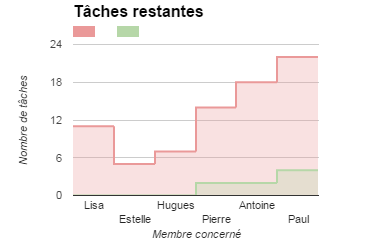
\includegraphics[width=10cm]{figures/taches_restantes.png}}
    \caption{Répartition des tâches par membres (responsabilités)}
\end{figure}

Le chef de projet et le responsable qualité ont un nombre de tâches légèrement supérieur du fait de leur statuts. Pour les autres membres du projet, le temps de travail a été réparti de la façon la plus équilibrée possible : certains responsables ont un peu plus de tâches, mais elles peuvent être plus rapides à effectuer que d’autres.
